\title{Math 239 Fall 2023 Tutorial Questions Week 10}

\date{2023 Nov. 23/24}
\maketitle

\begin{enumerate}
    \question{Planarity and Graph Complements} 
    \begin{enumerate}
        \item  For each $k\in\{ 5,6\}$ give two non-isomorphic graphs $G_1$ and $G_2$ with $k$ vertices each such that $G_1, G_2, \overline{G_1}, \overline{G_2}$ are planar. Prove they are planar(give a planar embedding) and give a one sentence proof that $G_1$ and $G_2$ are non-isomorphic. 
        \item Describe a graph $G$ where $\overline{G}$ and $G$ are both non-planar. 
     \end{enumerate}
    
    \question{Cartesian Product of Graphs} The \textit{Cartesian Product} of two graphs $G$ and $H$, denoted $G\square H$ is defined as 
    \[V(G\square H) = V(G) \times V(H)\]
    and if two vertices $(a_1, b_1)$ and $(a_2, b_2)$ are adjacent in $G \square H$ if and only if either 
    \begin{itemize}
        \item $a_1 = a_2$ and $b_1$ is adjacent to $b_2$ in H, or
        \item $b_1 = b_2$ and $a_1$ is adjacent to $a_2$ in G, 
    \end{itemize}
i.e.
    \[E(G\square H) = \{(a_1,b_1)(a_2,b_2): a_1 = a_2 \text{ and } b_1b_2\in E(H)\text{, or, }a_1a_2 \in E(G) \text{ and } b_1 = b_2\}\]
    \begin{enumerate}
        \item Suppose that $\phi_1$ is a $k$-coloring of $G$ (assigning colors $\{1,\cdots,k\}$ ) and  $\phi_2$ is a $k$-coloring of $H$ (assigning colors $\{1,\cdots,k\}$ ) for some positive integer $k$. Define\[\phi((a,b)) := \phi_1(a) + \phi_2(b)\mod{k}.\]
        Prove that $\phi$ is a $k$-coloring of $G\square H$.
        \item Deduce that if $G$ is $k_1$-colorable and $H$ is $k_2$-colorable, then $G\square H$ is $\max \{k_1, k_2\}$-colorable.
    \end{enumerate}

    
    \question{Graph Coloring} Let $k \ge 1$. Let $G$ be a graph where every nonempty subgraph has a vertex of degree at most $k$. Prove that $G$ is $(k + 1)$-colourable. Find an example of $G$ where $G$ is not $k$-colourable.

    
    \question{A Second Planarity Question} Determine whether or not each of the following graphs is planar. If so, give a planar embed- ding. If not, exhibit an edge subdivision of $K_5$ or $K_{3,3}$ in the graph.
    \begin{center}
    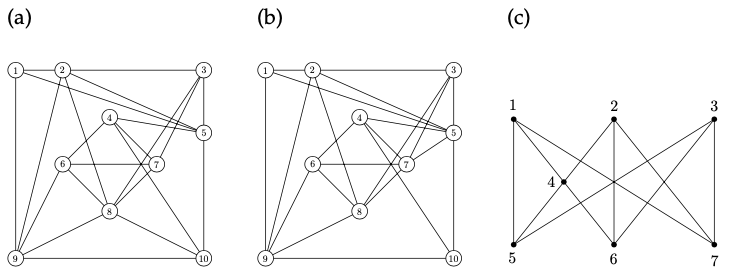
\includegraphics[scale=0.4]{t10q4drawings.png}
    \end{center}
    
    % \newpage
    
    \question{Bonus Question: Spectral Graph Theory}
    The Laplacian operator on $\mathbb{R}^n$, which acts on functions $\mathbb{R}^n \to \mathbb{R}$ by sending $f$ to $\Delta f = \sum_{i = 1}^n \frac{\partial^2 f}{\partial x_i^2}$. The Laplacian operator notionally measures how much $f$ at $p$ differs from points near $p$. It turns out this plays a large role in a theory of mathematics called spectral theory, which is concerned with finding functions $f$ such that $\Delta f = \lambda f$ (so-called ``eigenfunctions").

    There is a graph theory equivalent of the Laplacian. Let $G$ be a graph with $n$ vertices, labelled $1 , \cdots , n$. Then Define the \textbf{degree matrix} $D_G$ of $G$ as the $n \times n$ matrix
    \begin{align*}
        D_G(i,j) = \begin{cases}
            \deg (v_i) & \text{ if } i=j,\\
            0 & \text{ else}.
        \end{cases}
    \end{align*}
    Define as well the \textbf{adjacency matrix} $A_G$ of $G$ as the (symmetric) $n \times n$ matrix
    \begin{align*}
        A_G(i,j) = \begin{cases}
            -1 & \text{ if } v_i v_j \in E,\\
            0 & \text{ else}.
        \end{cases}
    \end{align*}
    Now finally define the \textbf{graph Laplacian} of $G$ as $L = L_G = D_G - A_G$. Since this is an $n \times n$ real symmetric matrix, there are $n$ real eigenvalues (counted with multiplicity). This is exactly the provenance of \textbf{spectral graph theory}. We call the multiset of eigenvalues the \textbf{spectrum} of a graph, and often write them in increasing order $\lambda_1 \leq \cdots \leq \lambda_n$ (so that $\lambda_1$ is the lowest eigenvalue of $G$).
    \begin{enumerate}
        \item Argue that for any $G$ then $L (1, \cdots, 1)^T = 0$, and so $0$ is always an eigenvalue of $G$.
        \item Find the spectrum of $K_n$, $K_{n,n}$, $P_n$, $C_n$, the star graph $S_n$, and the $n$-cube $Q_n$.
        \item Prove that if $G$ is connected then $\lambda_1> 0$.  Further show that if $\lambda_i = 0$ and $\lambda_{i+1} \neq 0$ then $G$ has exactly $i+1$ connected components.
    \end{enumerate}
\end{enumerate}